\documentclass{article}
\linespread{0.7}
\usepackage[a4paper, margin=3mm, landscape]{geometry}
\usepackage{multicol}
\usepackage{xcolor}
\usepackage{enumitem}
\usepackage{amsmath}
\usepackage{amsfonts}
\usepackage{listings}
\usepackage{soul}
\usepackage{graphicx}

\pdfinfo{
    /Title (template.pdf)
    /Creator (TeX)
    /Producer (pdfTeX 1.40.0)
    /Author (securespider)
    /Subject (cs3103)
    /Keywords (cheatsheet, pdf, cs3103)
}

\graphicspath{ {./img/} }

\pagestyle{empty}
\setcounter{secnumdepth}{0}
\setlength{\columnseprule}{0.25pt}

% Redefine section commands to use less space
\makeatletter
\renewcommand{\section}{\@startsection{section}{1}{0mm}%
    {-1ex plus -.5ex minus -.2ex}%
    {0.5ex plus .2ex}%x
{\normalfont\large\bfseries}}
\renewcommand{\subsection}{\@startsection{subsection}{2}{0mm}%
    {-1explus -.5ex minus -.2ex}%
    {0.5ex plus .2ex}%
{\normalfont\normalsize\bfseries}}
\renewcommand{\subsubsection}{\@startsection{subsubsection}{3}{0mm}%
    {-1ex plus -.5ex minus -.2ex}%
    {1ex plus .2ex}%
{\normalfont\small\bfseries}}%
\makeatother

% Adjust spacing for all itemize/enumerate
\setlength{\leftmargini}{0.5cm}
\setlength{\leftmarginii}{0.5cm}
\setlist[itemize,1]{leftmargin=2mm,labelindent=1mm,labelsep=1mm}
\setlist[itemize,2]{leftmargin=2mm,labelindent=1mm,labelsep=1mm}

% Font
\renewcommand{\familydefault}{\sfdefault}

% Define colors for math formulas
\definecolor{myblue}{cmyk}{1,.72,0,.38}
\everymath\expandafter{\the\everymath \color{myblue}}

% Custom command for keywords
\definecolor{highlight}{RGB}{251,243,218}
\newcommand{\keyword}[2][]{\sethlcolor{highlight}\hl{\textbf{#2}} #1 - }
\newcommand{\ilkeyword}[1]{\sethlcolor{highlight}\hl{\textbf{#1}}}

% Define colors and style for code
\definecolor{codegreen}{rgb}{0,0.6,0}
\definecolor{codegray}{rgb}{0.5,0.5,0.5}
\definecolor{codered}{HTML}{CC241D}
\definecolor{backcolor}{rgb}{0.95,0.95,0.95}
\lstdefinestyle{codestyle}{
    backgroundcolor = \color{backcolor},
    commentstyle = \color{codegray},
    keywordstyle = \color{codered},
    stringstyle = \color{codegreen},
    basicstyle = \ttfamily,
    breakatwhitespace = false,
    showstringspaces = false,
    breaklines = true,
    showtabs = false,
    tabsize = 2
}
\lstset{style = codestyle}

% -----------------------------------------------------------------------
\begin{document}
\begin{multicols*}{4}
\footnotesize

% Title box
\begin{center}
    \fbox{
        \parbox{0.8\linewidth}{
            \centering \textcolor{black}{
                {\Large\textbf{CS3103}} \\
                \normalsize{Computer Networks Practice}} \\
                {\footnotesize \textcolor{gray}{github.com/securespider}}
        }
    }
\end{center}
\section{01. Intro}
\subsection{Revision}
\begin{description}
	\item[DHCP]{Getting IP address, gateway and DNS server}
	\begin{itemize}
		\item Uses DHCP Discover, Offer, Request, Acknowledge
		\item DHCP renew to  
		\item DHCP release if no longer in use
	\end{itemize}
	\item[ARP]{MAC address from IP address}
	\begin{itemize}
		\item ARP Query, Reply (only within same network)
	\end{itemize}
	\item[DNS]{Mechanism to get IP from URL}
	\begin{itemize}
		\item DNS query, recursive DNS/resolvers, Authoritative DNS
	\end{itemize}
	\item[HTTP]{Application layer TCP connection}
	\begin{itemize}
		\item HTTP Request, Response
	\end{itemize}
	\item[Subnet]{Interface with same subnet-ID}
	\begin{itemize}
		\item Classful vs Classless
		\item Security, performance(reduce broadcasts and collisions)
	\end{itemize}
	\item[Supernet]{Merging small networks into larger network w single prefix}
	\item[NAT]{Network Address Translation: Changing private addresses to public addresses}
\end{description}
\section{02. ARP/DHCP}
\subsection{ARP}
\begin{description}
	\item[Proxy ARP]{Host or router responds to ARP request for host on other networks}
	\item[Gratuitous ARP]{Sends ARP request for its own IP}
	\begin{itemize}
		\item Detect if there is other host sharing same IP address
		\item Utilised after IP assigned by DHCP
	\end{itemize}
\end{description}
\subsubsection{Vulnerability (ARP Poisoning)}
\begin{itemize}
	\item Forgery of requests and reply
	\item Stateless protocol: Replies can be sent without requests
	\item \hl{Must} update ARP cache with new reply
\end{itemize}
\subsection{DHCP}
\begin{itemize}
	\item Allocation of IP addresses from a pool
	\begin{itemize}
		\item Static configuration for indefinite time (routers)
		\item Automatic configuration 
		\item Dynamic configuration for specific duration (loans)
	\end{itemize}
	\item Server waits on UDP 67 and Client communicates on UDP 68
\end{itemize}
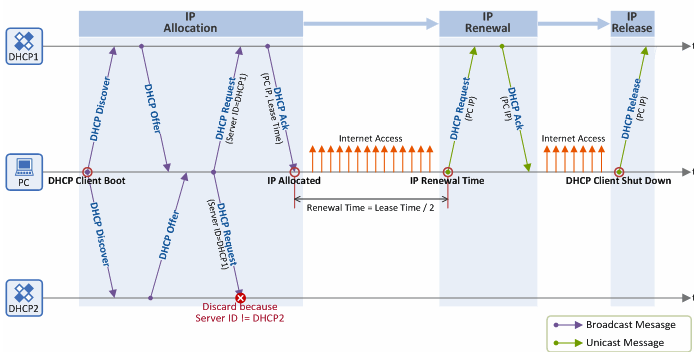
\includegraphics[scale=0.3]{02-dhcp}
\subsubsection{Relay Agent}
\begin{itemize}
	\item Device that forwards requests to one of more DHCP server
	\begin{itemize}
		\item DHCP server does not have to be in same subnet
	\end{itemize}
	\item Places its IP address in \hl{router-address field}
	\item Increments hop count by 1
\end{itemize}
\subsubsection{Packet Format}
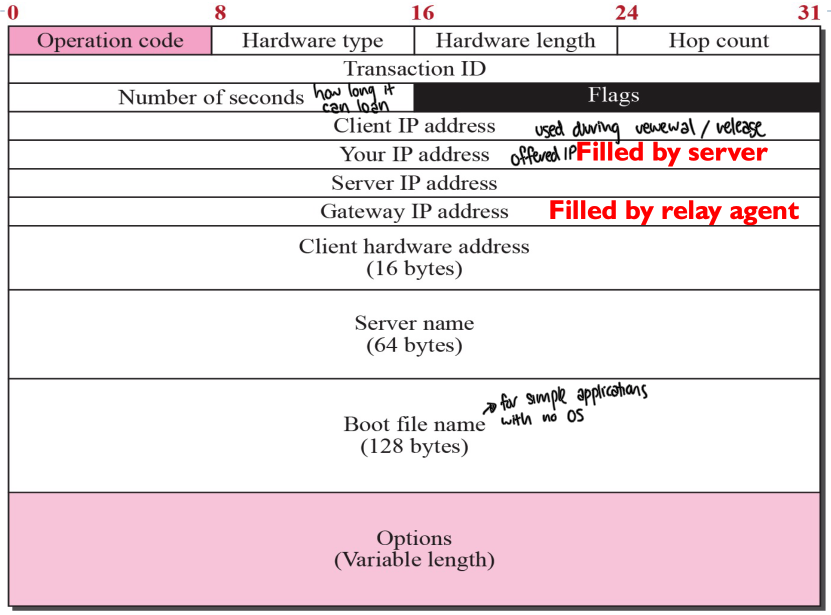
\includegraphics[scale=0.2]{02-dhcp-packet}
\begin{description}
	\item[Field OP]{1 - request, 2 - reply}
	\item[HTYPE and HLEN]{Network hardware type and length of address}
	\begin{itemize}
		\item Ethernet is type 1 and length 6
	\end{itemize}
	\item[Hops]{Initialised as 0 and increments whenever passing through another router}
	\item[Xid]{Transaction ID to match response to request}
	\item[Seconds]{Type since client boot}
	\item[Flags]{Indicate broadcast(1) and other reserved use}
	\begin{itemize}
		\item When client cannot accept unicast, MSB set to 1 (broadcast)
	\end{itemize}
	\item[..]{All known is field, the rest set to 0}
	\item[Option]{Used mostly in reply for addi info to client}
	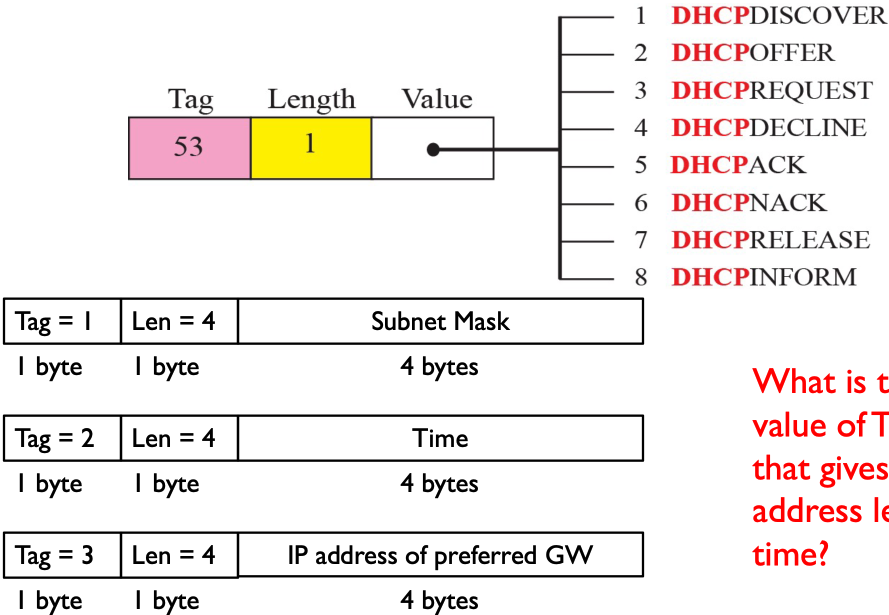
\includegraphics[scale=0.2]{02-option-format}
\end{description}
\subsubsection{Server}
\begin{itemize}
	\item Server stores a (key, value) pair for each client
	\item Key identifies client (IP-subnet and MAC address)
	\item Value is IP address assigned and lease time
	\begin{itemize}
		\item Leased time represented in seconds in relation to client clock
		\item Lease expiration = time client sent DHCPReq + Lease duration DHCPAck
		\item 0xFFFFFFFF == infinite time
	\end{itemize}
\end{itemize}
\subsubsection{Process}
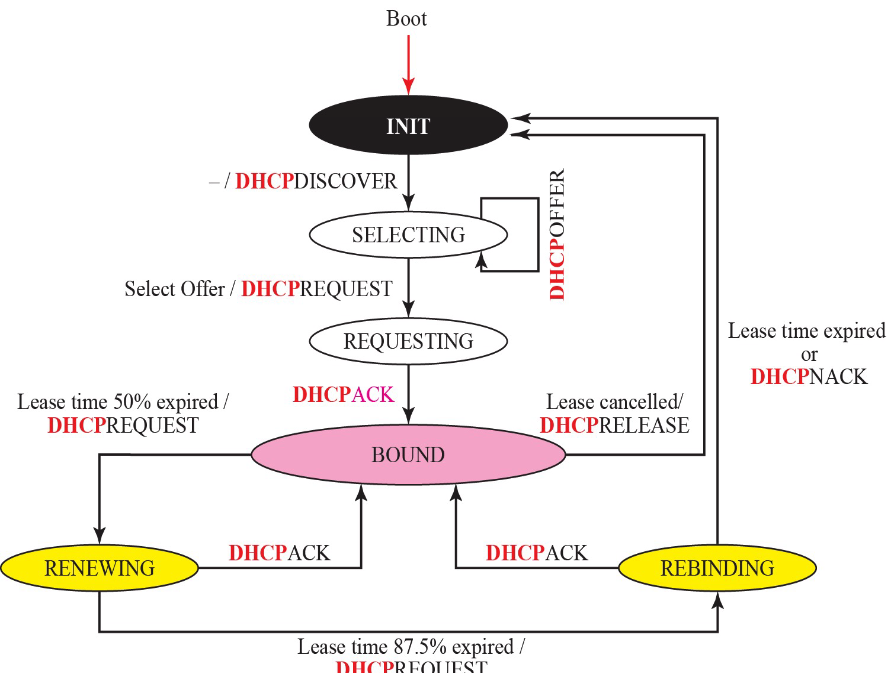
\includegraphics[scale=0.2]{02-transition-diagram}
\begin{itemize}
	\item Rebinding may have diff info vs Renew = same info
\end{itemize}

\section{04. Network Application}
\begin{description}
	\item[Client-server]{Dedicated server with perma IP and ports}
	\item[P2P]{Arbitary end system directly comunicate and serve each other}
\end{description}
\subsection{Transport}
\subsubsection{Socket}
\begin{itemize}
	\item Interface between application and transport layer
	\item OS-controlled interface via IP address and port no
\end{itemize}
\subsubsection{Protocol services}
\begin{description}
	\item[TCP]{Reliable transport btw sending and receiving process}
	\begin{itemize}
		\item Flow, congestion control
		\item Does not provide timing, min throughput guarantee, security
		\item Connection oriented (3 way handshake)
	\end{itemize}
	\item[UDP]{Unreliable data transfer but faster}
	\begin{itemize}
		\item Only demultiplexing provided: Passing to the correct app
		\item Used for streaming where packet reliability not very impt
		\item Used when application wants to manage their own protocol
	\end{itemize}
	\item[SSL]{Encrypted TCP connection with data integrity and endpoint auth}
	\begin{itemize}
		\item SSL is at app layer which contains libraries to interact directly TCP
	\end{itemize}
\end{description}
\subsection{HTTP}
\begin{itemize}
	\item Stateless using TCP
\end{itemize}
\subsubsection{Persistence}
\begin{description}
	\item[Non persistence]{Server terminates connectoin after trf file}
	\begin{itemize}
		\item Response time = 2 RTT + transmit time
		\item RTT = time taken for small packet from client to server and back
	\end{itemize}
	\item[Pers - pipeline]{$\geq 1$ RTT per referenced object}
	\item[Pers + pipeline]{Possibly one RTT for all referenced object}
\end{description}
\subsection{Components}
\begin{enumerate}
	\item User agents/Mail readers
	\item Message transfer agents (SMTP port 25)
	\item Message Access Agents (POP3- port 110 and IMAP4 port 143)























\end{multicols*}
\end{document}
